\documentclass[11pt]{article}

\usepackage[margin=1in]{geometry}
\usepackage{graphicx}
\usepackage{booktabs}
\usepackage{microtype}
\usepackage[hidelinks]{hyperref}
\usepackage{xurl}
\usepackage{caption}
\captionsetup{font=small, labelfont=bf}

\graphicspath{{figs/}}

\title{From Buildout Story to Backlash Story: Media Sentiment Toward
Data Centers in a Six-Technology Benchmark, 2015--2026}
\author{Ganesh Hegde\\
\small KETOS Inc.\\
\small \texttt{ganesh@ketos.co}}
\date{July 2026}

\begin{document}
\maketitle

\begin{abstract}
English-language news coverage of data centers grew tenfold between January
2022 and June 2026 while its sentiment reversed sign. Using two
complementary sampling frames from GDELT, the Global Database of Events,
Language, and Tone (335,206 fulltext-mention articles and a census of
103,341 articles with the term in the headline frame), LLM classification of
8,100 sampled headlines, and a six-technology comparison corpus of 921,170
articles spanning 2015--2026, we measure the reversal and place it in
context. Net headline sentiment toward data centers fell from +54 points in
2022 to $-5$ points in the first half of 2026, with the first net-negative
month in March 2026. Among six infrastructure and technology buildouts (5G,
wind, solar, fracking, cryptocurrency mining, data centers), the data center
decline is the largest sustained tone decline from a net-positive starting
level, and unlike the 5G and wind episodes, which recovered within two to
four months of turning negative, it had not recovered as of June 2026.
Classifying outlets by type shows the negativity is stratified: local news
outlets run roughly 13 percentage points more negative than national outlets
throughout, and are the only outlet class whose net sentiment turned
sustainably negative; local and national series move together with no
detectable lead-lag. Thematically, coverage shifted from investment and
buildout (59\% of headlines in 2022, 27\% in 2026) toward community
opposition (5\% to 22\%) and energy, while water-related coverage grew 2.4x
from a small base. All data, code, prompts, and classification rubrics are
released for reproduction.
\end{abstract}

\section{Introduction}

Between 2022 and 2026, data centers moved from a specialist infrastructure
topic to a mainstream news subject. The share of global English-language news
coverage mentioning data centers grew 7.2x over the period, and the absolute
number of articles carrying the term in their headline frame grew from 838 to
9,120 per month. Over the same window, the sentiment of that coverage
reversed: headlines that in 2022 were dominated by investment announcements
were, by mid-2026, dominated by stories about community opposition, grid
strain, and environmental resources.

This paper measures that reversal quantitatively and asks three questions.
First, how large and how fast is the sentiment decline, measured
consistently over four and a half years? Second, how does it compare with
prior technology buildouts that attracted public controversy: 5G, wind
power, solar power, hydraulic fracturing, and cryptocurrency mining? Third,
what is the internal structure of the decline across outlet types and
coverage themes?

Our contributions are methodological and empirical. Methodologically, we
combine two GDELT sampling frames with LLM headline classification, publish
the full rubric and quality-control results, calibrate the LLM series
against GDELT's independent lexicon-based tone measure, and apply a uniform
promotional-content filter across all six technologies. Empirically, we
document (i) a +54 to $-5$ point net-sentiment reversal for data centers,
(ii) its position as the largest net-positive-to-negative tone decline among
the six technologies studied, (iii) a 13-point stratification between local
and national outlet negativity with no detectable lead-lag between them, and
(iv) a thematic rotation from buildout coverage toward community opposition,
energy, and, from a small base, water.

We deliberately frame the analysis descriptively. News sentiment is an
observable property of published coverage; we make no claims about the
accuracy of that coverage or the merits of the underlying projects, and the
patterns documented here are offered as measurements that any stakeholder,
including infrastructure developers, utilities, regulators, and journalists,
can use.

\section{Data and methods}

\subsection{Two GDELT frames}

All raw data come from the GDELT Project (Global Database of Events,
Language, and Tone) \cite{leetaru2013}, an open platform that monitors
print and web news media worldwide in over 100
languages and machine-codes each article it sees, extracting entities,
locations, themes, and a lexicon-based tone score, on a 15-minute update
cycle. We use two GDELT products: the DOC 2.0 API, which supports fulltext
search over the monitored article stream, and the Global Knowledge Graph
(GKG), which publishes per-article metadata including the article URL and
tone score and is mirrored on Google BigQuery. From these we construct two
sampling frames with different tradeoffs between recall and precision:

\begin{itemize}
\item \textbf{Fulltext frame.} All English-language articles matching
``data center(s)'' or ``datacenter(s)'' anywhere in the article, via the
GDELT DOC 2.0 API: 335,206 articles, January 2022 through June 2026. This
frame has high recall but includes articles that mention data centers only
in passing.
\item \textbf{Headline frame.} A census of articles whose URL slug
contains the term, built from the GDELT Global Knowledge Graph on BigQuery
(English-only; pattern \texttt{data[-\_]?cent(er|re)} applied to the URL
path): 103,341 unique articles over the same period. Requiring the term in
the headline frame selects articles that are \emph{about} data centers.
\end{itemize}

The two frames agree well on volume dynamics (Pearson $r=0.93$ between the
frames' monthly article volumes), and the headline frame's share of the fulltext frame rose from
16\% in 2022 to 48\% in the first half of 2026: when data centers appear in
coverage at all, they are increasingly the story rather than the backdrop.

\subsection{Headline sampling and LLM classification}

From the headline census we drew a seeded random sample of 150 articles per
month (8,100 total across 54 months; median 141 relevant per month after
filtering). Headline text was recovered by fetching live page titles (72\%
of the sample) or reconstructing them from URL slugs (28\%; 80\% in 2026 as
older pages disappear, a limitation discussed in
Section~\ref{sec:limitations}).

Each headline was classified by Claude Sonnet (Anthropic) \cite{claude}
against a committed rubric with three dimensions: relevance (94\% of sampled
headlines are relevant), sentiment toward data centers (positive, negative,
neutral), and one of eight themes (energy and grid; environment and water;
community opposition; investment and buildout; jobs and economy; policy and
regulation; technology and operations; other). The full rubric, prompts, and
per-headline labels are in the repository.

\textbf{Quality control.} A seeded 10\% subsample (400 headlines) was
re-classified independently with shuffled batch composition. Agreement was
98.8\% on relevance, 87.2\% on sentiment, and 92.8\% on theme. No
disagreement flipped a headline between positive and negative (all sentiment
disagreements involved the neutral class), and the resulting monthly
net-sentiment series differ by 0.8 percentage points on average.

\subsection{Six-technology comparison corpus}

To place the data center episode in context we built an analogous
headline-frame corpus for five other technologies over 2015--2026: 5G
(276,950 articles), wind power (227,118), solar power (108,798), hydraulic
fracturing (87,229), and cryptocurrency mining (26,033), for a comparison
corpus of 921,170 articles including data centers. For each technology we
classified a quarterly headline sample with the same rubric and pipeline
(1,827--1,840 headlines per technology; 9,187 total), and computed the
GDELT lexicon tone of every article in the corpus.

\textbf{Promotional-content filter.} Press-release wires and promotional
content are unevenly distributed across technologies and time; unfiltered,
they produced a spurious positive tone spike in 2025 cryptocurrency coverage
of which 22\% proved promotional. We therefore excluded PR-wire and
promotional content uniformly across all six technologies (the
cryptocurrency example is the largest correction: article-count-weighted
mean tone $+1.03$ raw versus $+0.09$ filtered). Raw series are retained in
the repository as an annex. The data center finding is strengthened, not
weakened, by the filter.

\subsection{Calibration against GDELT tone}
\label{sec:calibration}

The LLM net-sentiment series and GDELT's lexicon-based tone are independent
measurements: the former reads 150 sampled headlines per month, the latter
averages a dictionary score over every article in the census. Their
agreement is a check on both. Table~\ref{tab:calibration} reports Pearson
correlations computed by the committed calibration script.

\begin{table}[t]
\centering
\caption{Pearson correlation between LLM net headline sentiment and
article-count-weighted GDELT tone. Quarterly aggregation; the data center
series is also shown monthly.}
\label{tab:calibration}
\begin{tabular}{lcc}
\toprule
Technology & Periods & $r$ \\
\midrule
Data centers (monthly) & 54 & 0.85 \\
Data centers (quarterly) & 18 & 0.92 \\
Cryptocurrency mining & 46 & 0.66 \\
5G & 46 & 0.60 \\
Wind power & 46 & 0.55 \\
Solar power & 46 & 0.38 \\
Hydraulic fracturing & 46 & $-0.04$ \\
\bottomrule
\end{tabular}
\end{table}

Calibration is strongest where sentiment actually moves: the data center
series, with the largest dynamic range, correlates at $r=0.92$ quarterly.
Fracking, whose tone is persistently negative with little variation over
2015--2026, shows no correlation; when a series spends a decade in a flat
regime, sampling noise dominates both measures and correlation is not an
informative validity check. We therefore read Table~\ref{tab:calibration}
as validating the method in exactly the regimes where we use it to make
claims about change.

\subsection{Outlet-type classification}

For the outlet-structure analysis (Section~\ref{sec:outlets}) we classified
all 1,979 unique domains in the classified sample into five outlet types
(local, national, trade, wire/PR, other) using an LLM pass over the domain
name and sample headlines, against a committed rubric. Locality-sounding
PR-syndication networks were identified via duplicate press-release
headlines across domains and assigned to wire/PR. An independent 10\%
double-classification (197 domains) agreed 92.9\% overall and 100\% on the
local-versus-not distinction that the analysis depends on. Wire/PR (1,716
relevant headlines) and unclassifiable (93) rows are excluded from
outlet-level series, leaving 1,980 local, 1,434 national, and 2,387 trade
relevant headlines.

\section{Results}

\subsection{The reversal}

Net headline sentiment (share positive minus share negative, among relevant
headlines) declined monotonically at annual resolution: $+54$ points in
2022, $+49$ in 2023, $+48$ in 2024, $+28$ in 2025, and $-5$ in the first
half of 2026 (Figure~\ref{fig:net}). The first net-negative month was March
2026; the deepest month in the series is May 2026 at $-18$ points. The
series peaked in January 2022 at $+70$ points.

GDELT's independent lexicon tone over the full census confirms the shape:
tone fell from $+1.09$ in January 2022 to $-0.35$ in June 2026, first
crossing zero in March 2026, the same month as the LLM series
(Figure~\ref{fig:xval}). Coverage volume grew 10.9x over the same window
(838 to 9,120 headline-frame articles per month), so the negative turn is
not a thinning of coverage but a change in the composition of a rapidly
expanding coverage base.

\begin{figure}[t]
\centering
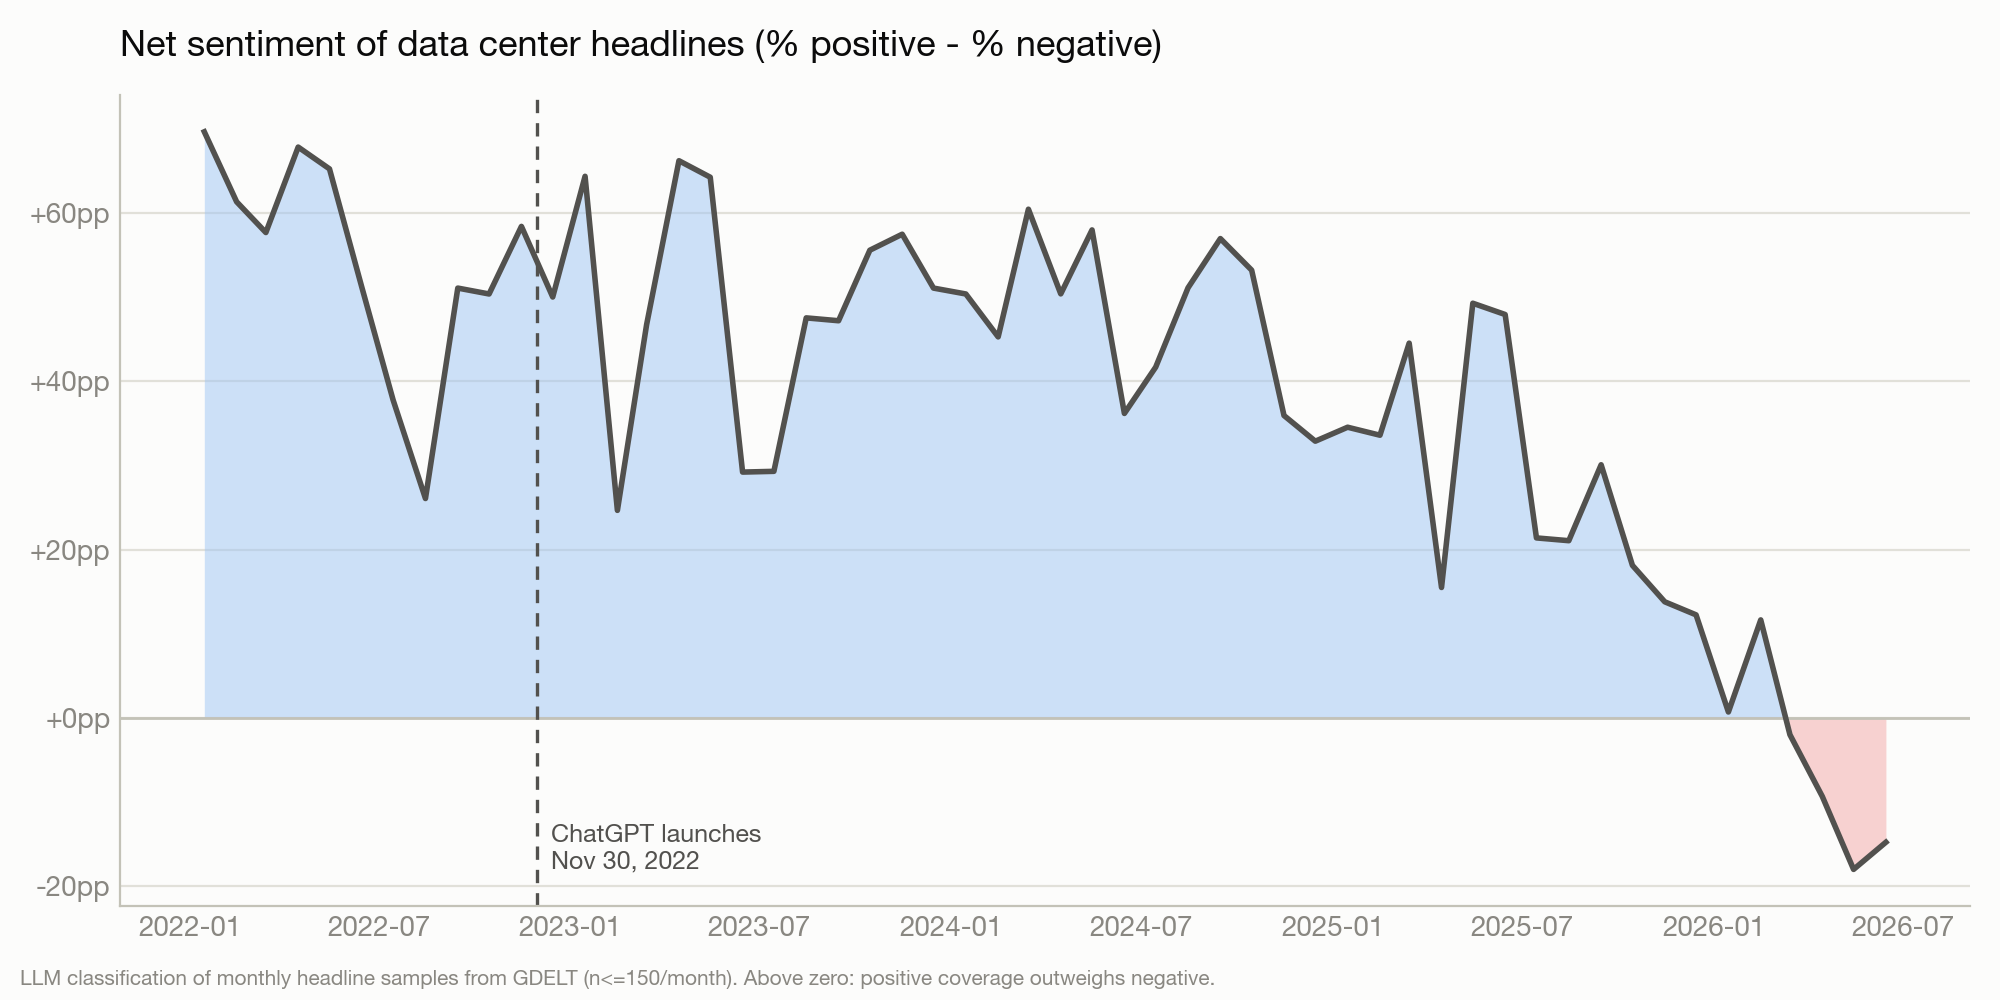
\includegraphics[width=\textwidth]{04_net_sentiment.png}
\caption{Net sentiment of data center headlines (share positive minus share
negative), monthly, from LLM classification of 150 sampled headlines per
month. The series first turns negative in March 2026.}
\label{fig:net}
\end{figure}

\begin{figure}[t]
\centering
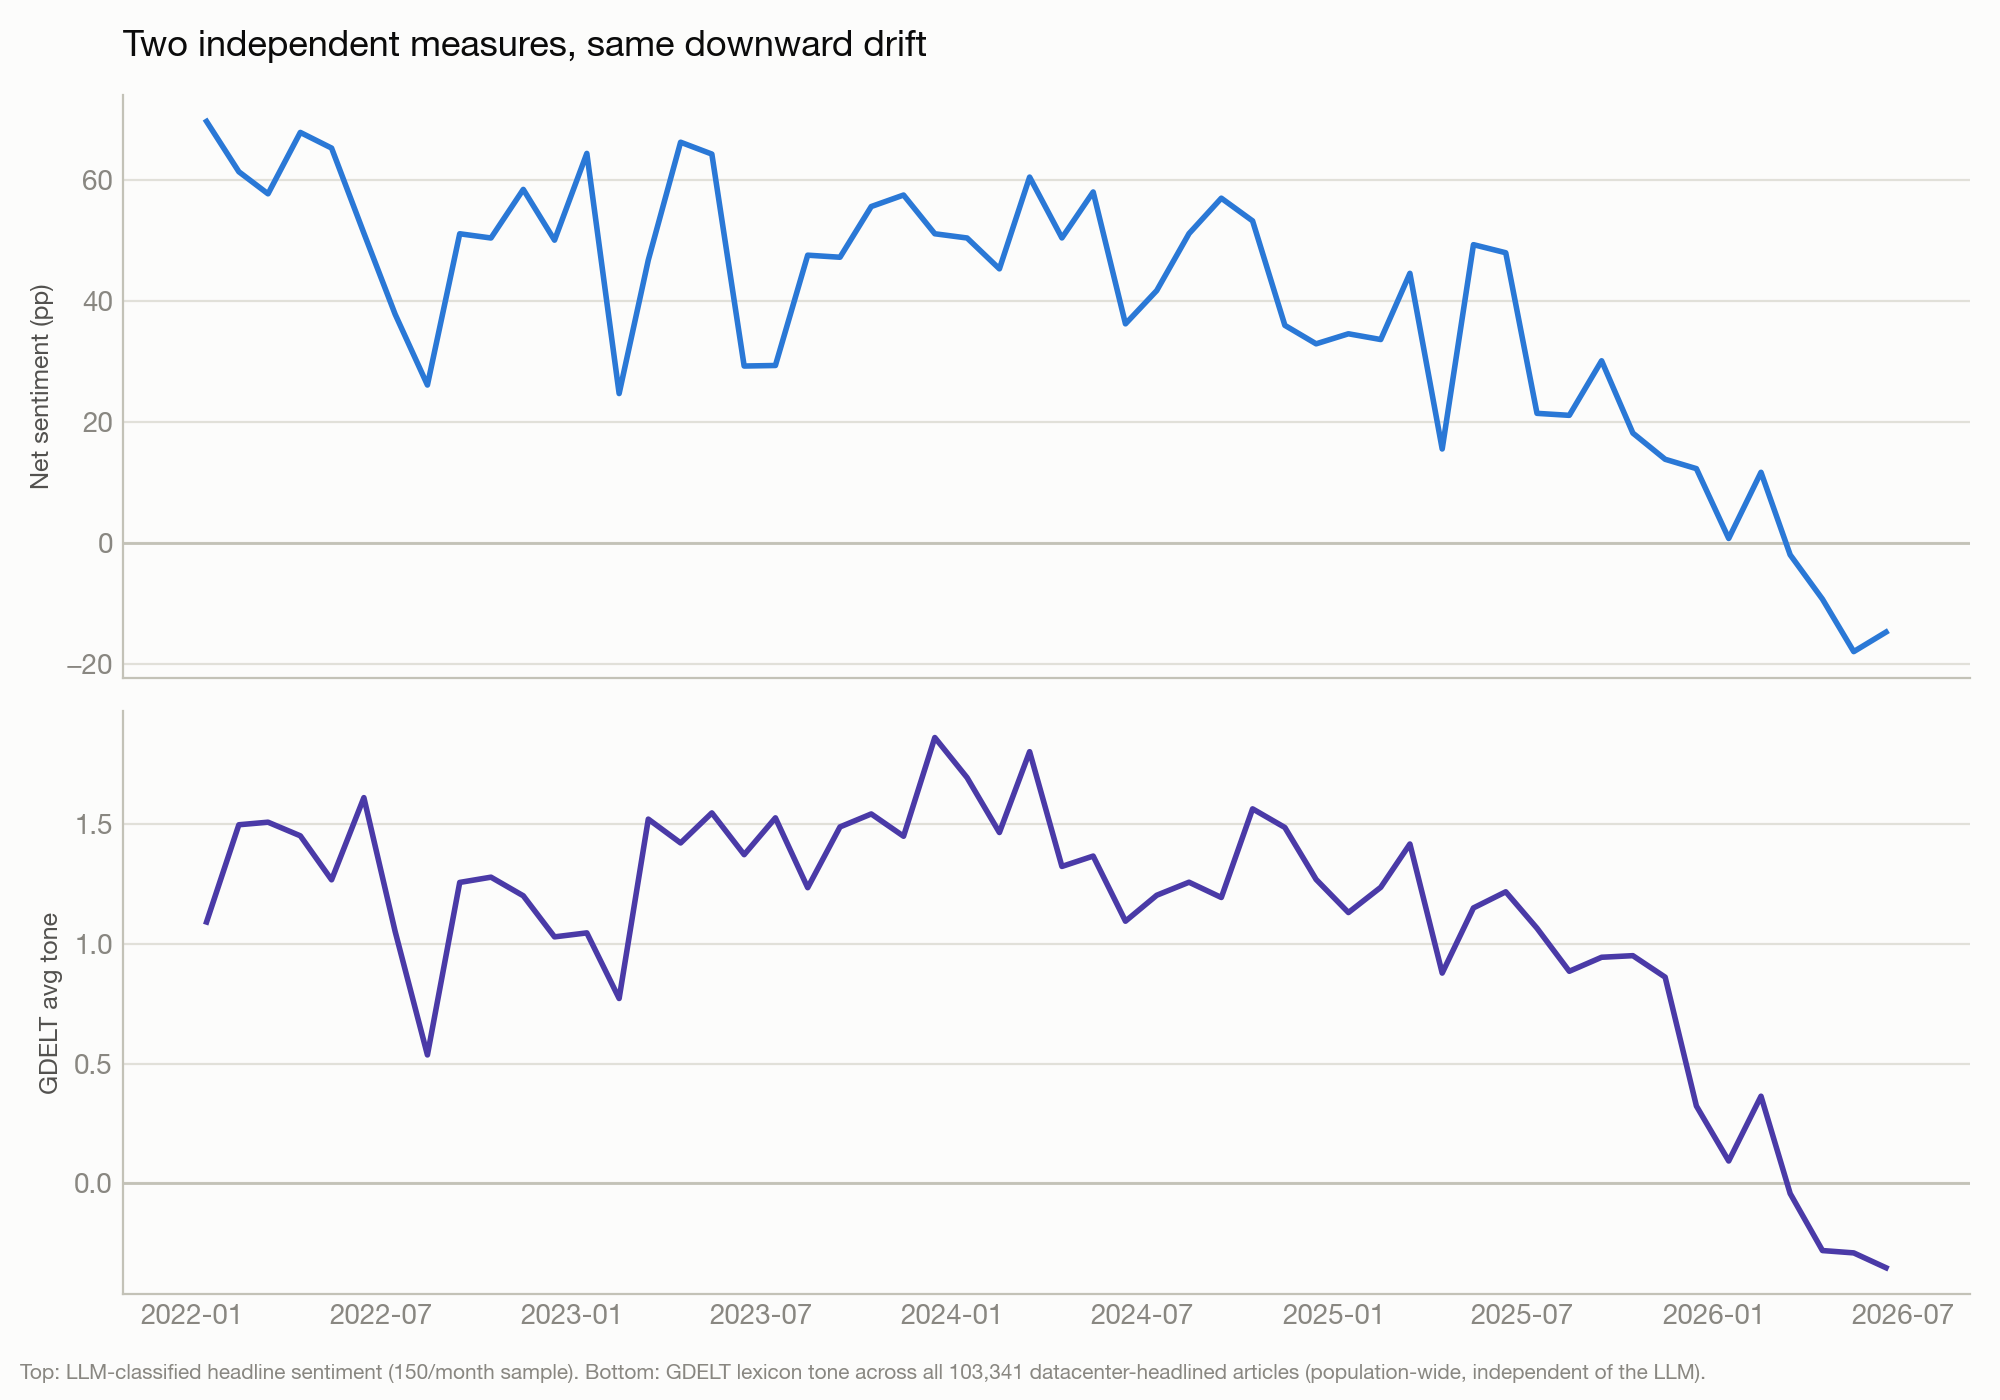
\includegraphics[width=\textwidth]{05_tone_crossvalidation.png}
\caption{Cross-validation: LLM net sentiment (top, monthly sample) and
GDELT lexicon tone over all 103,341 census articles (bottom). The measures
are independent; both cross zero in March 2026.}
\label{fig:xval}
\end{figure}

\subsection{Six-technology benchmark}
\label{sec:benchmark}

Figure~\ref{fig:aligned} aligns the six technologies' tone series around
their coverage takeoffs, and Figure~\ref{fig:flip} summarizes the timing.
We define \emph{takeoff} as the first month in which a three-month coverage
window sustains at least twice the median of all prior months (minimum 500
articles), and a \emph{flip} as two consecutive smoothed months of negative
tone following the pre-decline goodwill peak.

Three patterns emerge. First, the magnitude: measured as the largest
18-month decline in smoothed tone, data centers fell 1.42 tone points from
a $+1.26$ starting level. Cryptocurrency mining's raw decline is nominally
larger (1.73 points) but starts from an approximately neutral level
($-0.03$); the data center episode is the largest decline from a clearly
net-positive starting level, i.e., the deepest measured loss of prior
goodwill among the six.

Second, the timing: data center tone flipped negative 26 months after its
goodwill peak. The comparable figures are 28 months for 5G and 38 months
for wind; fracking was net-negative throughout the observation window and
solar never flipped.

Third, and most distinctive, the recovery: 5G tone recovered to positive
four months after flipping, and wind two months after. Data center tone had
not recovered as of June 2026, the end of our window. Among the six
technologies, only fracking (persistently negative) offers a precedent
for a flip that is not reversed within a few months (cryptocurrency mining
recovered after five), and neither fracking nor cryptocurrency entered its
decline from a strongly positive baseline. Whether the
data center series follows the 5G/wind pattern (fast reversion) or
establishes a new persistent regime is, at this writing, an open empirical
question that the released pipeline can track.

\begin{figure}[t]
\centering

\includegraphics[width=\textwidth]{08_backlash_aligned.png}
\caption{GDELT tone aligned on coverage takeoff for the three technologies
with a detected takeoff (data centers, 5G, cryptocurrency mining), with
solar's full-period range shown as a band for scale; promotional content
removed uniformly. Wind, solar, and fracking never met the takeoff
threshold.}
\label{fig:aligned}
\end{figure}

\begin{figure}[t]
\centering

\includegraphics[width=\textwidth]{09_time_to_flip.png}
\caption{Months from pre-decline goodwill peak to sustained negative tone
(flip), and from flip to recovery where applicable.}
\label{fig:flip}
\end{figure}

\subsection{Outlet structure: a level gap, not a diffusion lag}
\label{sec:outlets}

A natural hypothesis is that negativity starts in local outlets covering
siting disputes and later diffuses to national coverage. The data support
half of that picture. Local outlets are substantially more negative
throughout: their mean quarterly negative share is 30.8\% versus 18.0\% for
national outlets, and in 2026-Q2 the gap was 52.2\% versus 31.5\% (trade
press: 27.8\%). Local outlets are also the only class whose net sentiment
flipped sustainably negative (2025-Q3); national and trade net sentiment
remained positive through 2026-Q2 (Figure~\ref{fig:outlets}).

However, we find no evidence of a lead-lag: the Pearson cross-correlation
between
local and national negative shares peaks at lag zero ($r=0.74$ quarterly
and $r=0.68$ monthly, in each case exceeding every realization of an
exhaustive circular-shift null, i.e.\ $p<0.06$ quarterly and $p<0.02$
monthly at the test's resolution), with symmetric decay at adjacent lags. At monthly resolution, local and national negativity move
together; what distinguishes local coverage is its level, not its timing.
For anyone monitoring coverage as a leading indicator, this suggests
watching how negative local coverage \emph{is}, rather than expecting it to
provide months of advance warning of national coverage.

\begin{figure}[t]
\centering
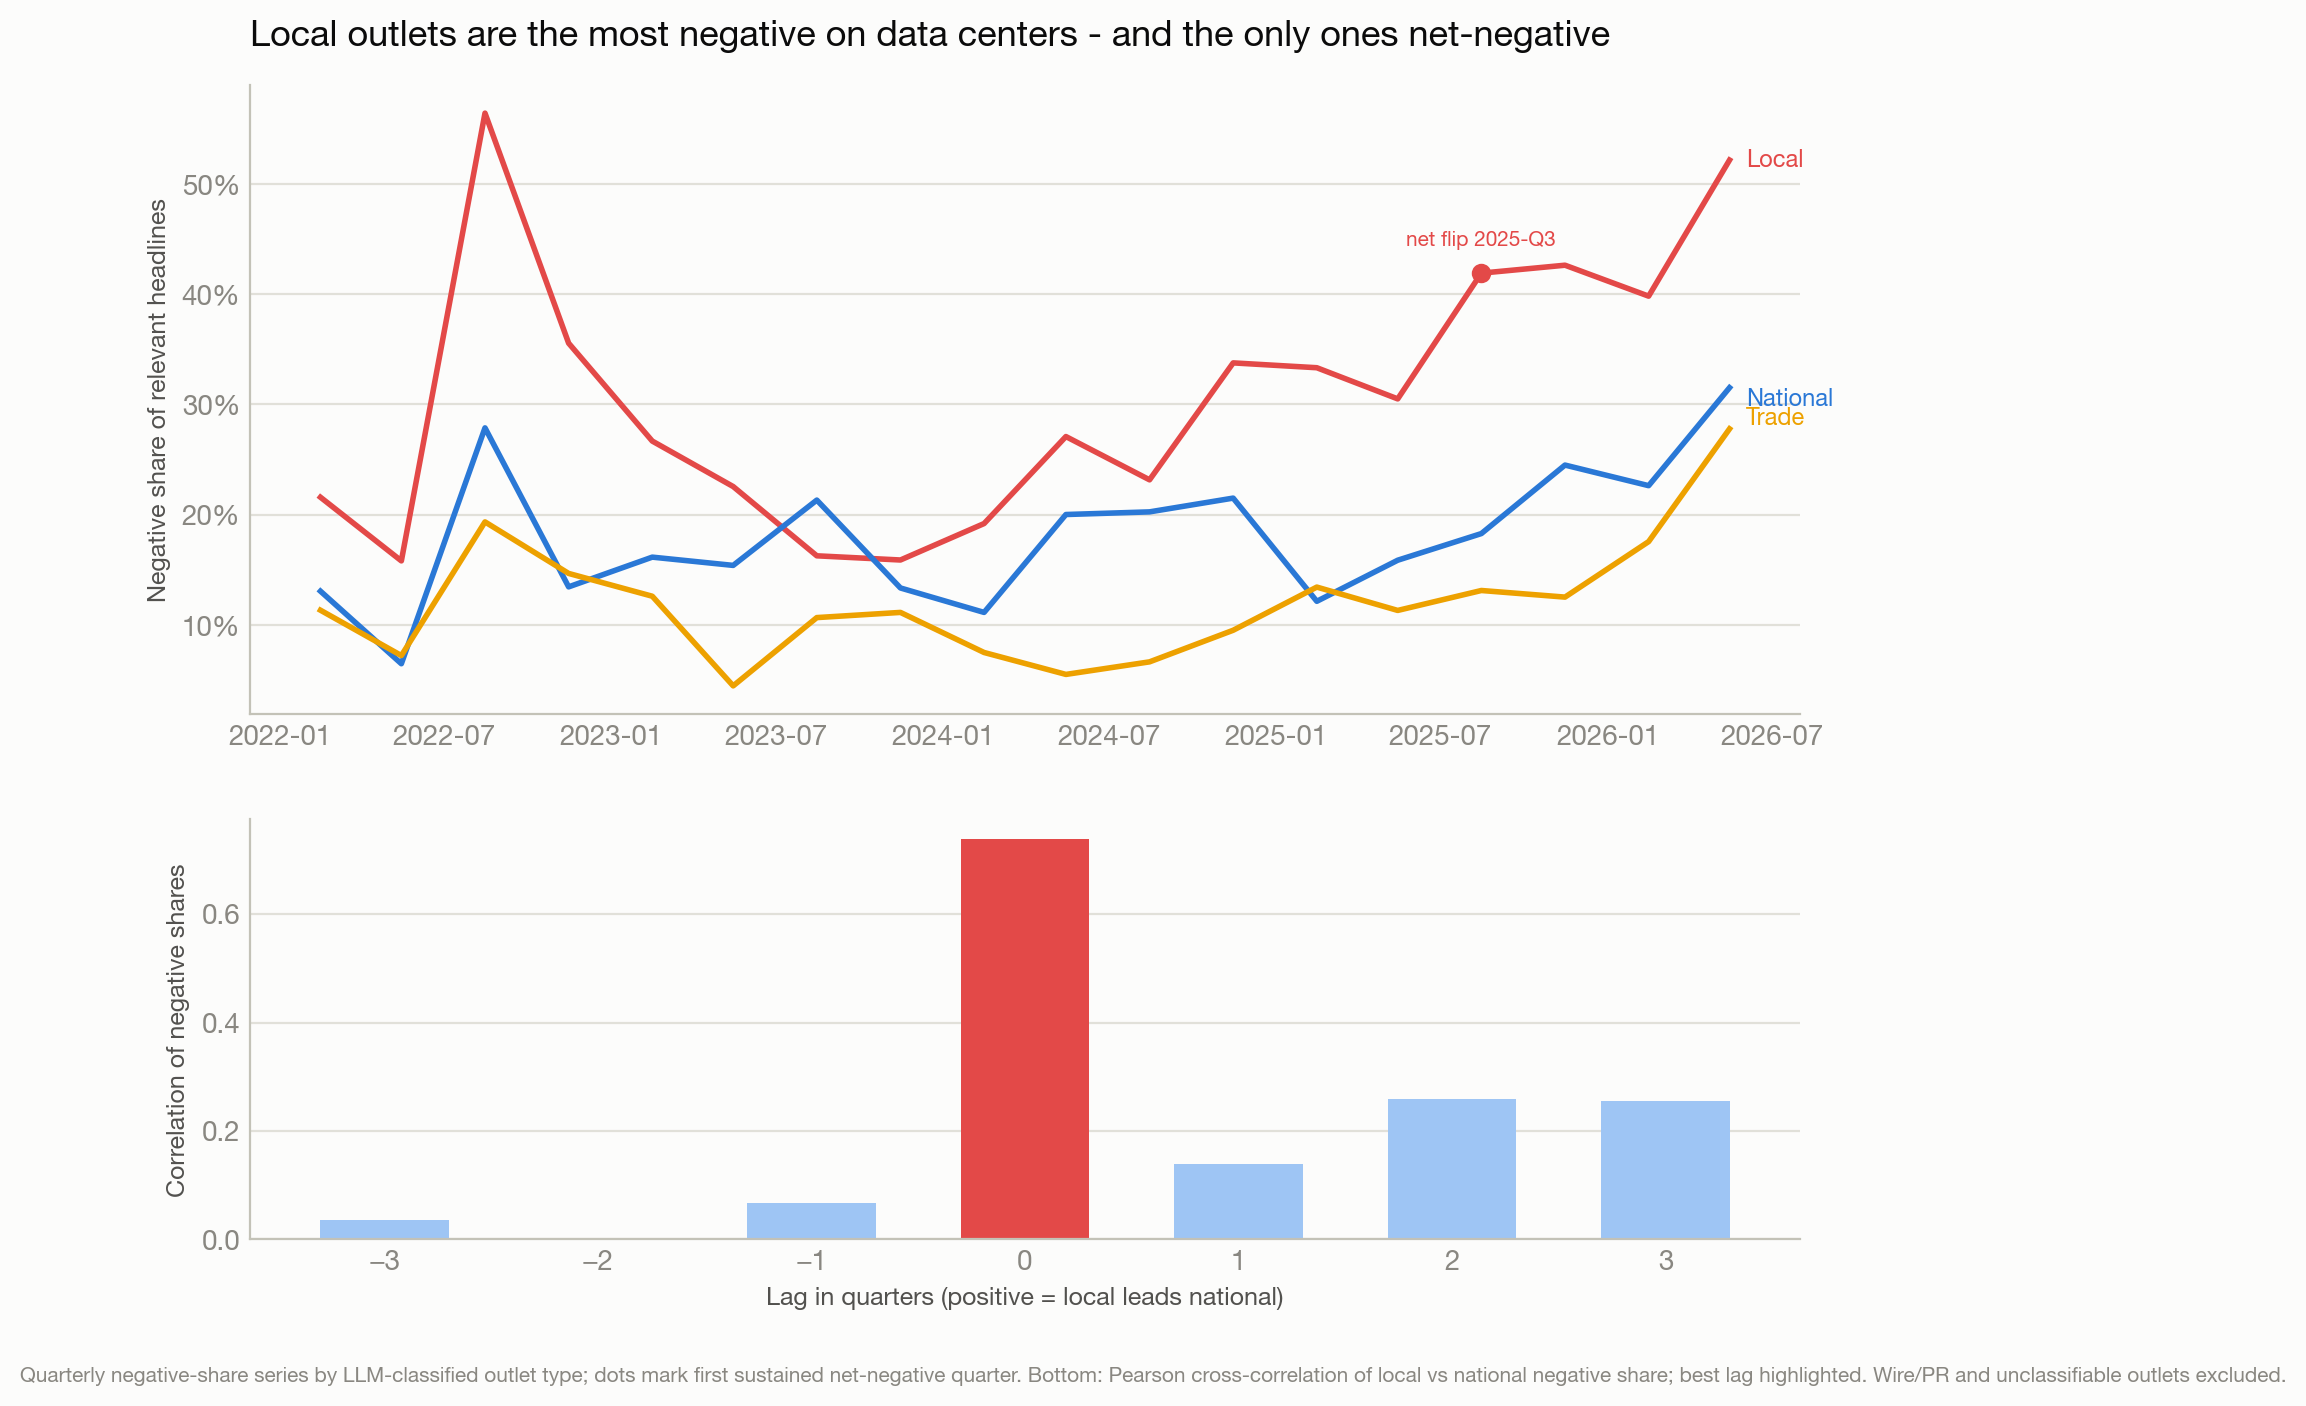
\includegraphics[width=\textwidth]{12_local_vs_national.png}
\caption{Top: quarterly negative share of relevant headlines by outlet
type; the dot marks the first sustained net-negative quarter (local only).
Bottom: cross-correlation of local versus national negative share by lag;
the maximum is at lag zero.}
\label{fig:outlets}
\end{figure}

\subsection{Thematic rotation, and water}
\label{sec:themes}

The theme mix explains what changed. Investment-and-buildout headlines fell
from 59\% of relevant coverage in 2022 to 27\% in 2026. Community
opposition rose from 5\% to 22\%, and energy-and-grid coverage peaked at
29\% of headlines in October 2024. Among negative headlines specifically,
community opposition is the largest theme in both the early (2022--2023)
and late (2025 through June 2026) periods, followed in the late period by
energy and grid.

Water-related coverage warrants separate treatment because it is measured
here two ways (Figure~\ref{fig:water}). As a classified theme (single label
per headline), environment-and-water holds a roughly flat 5--6\% share
across the period; but because each headline receives exactly one theme,
the rapid growth of the energy theme mechanically crowds the water label in
stories that touch both. Keyword measurement over the full census avoids
this: the share of census articles with water-related terms in the headline
slug (water, drought, aquifer, groundwater, wastewater) grew from 1.4\% in
2022--2023 to 3.2\% in 2025 through June 2026, a 2.4x increase, slightly
faster than the parallel energy-keyword share (2.1x) though from a base
roughly five times smaller. Water is the third-ranked theme among negative
headlines in both periods, behind community opposition and energy. The
keyword proxy was validated against fetched titles (recall 0.95, precision
0.83, with most nominal false positives traced to title-fetch failures
rather than slug errors).

\begin{figure}[t]
\centering
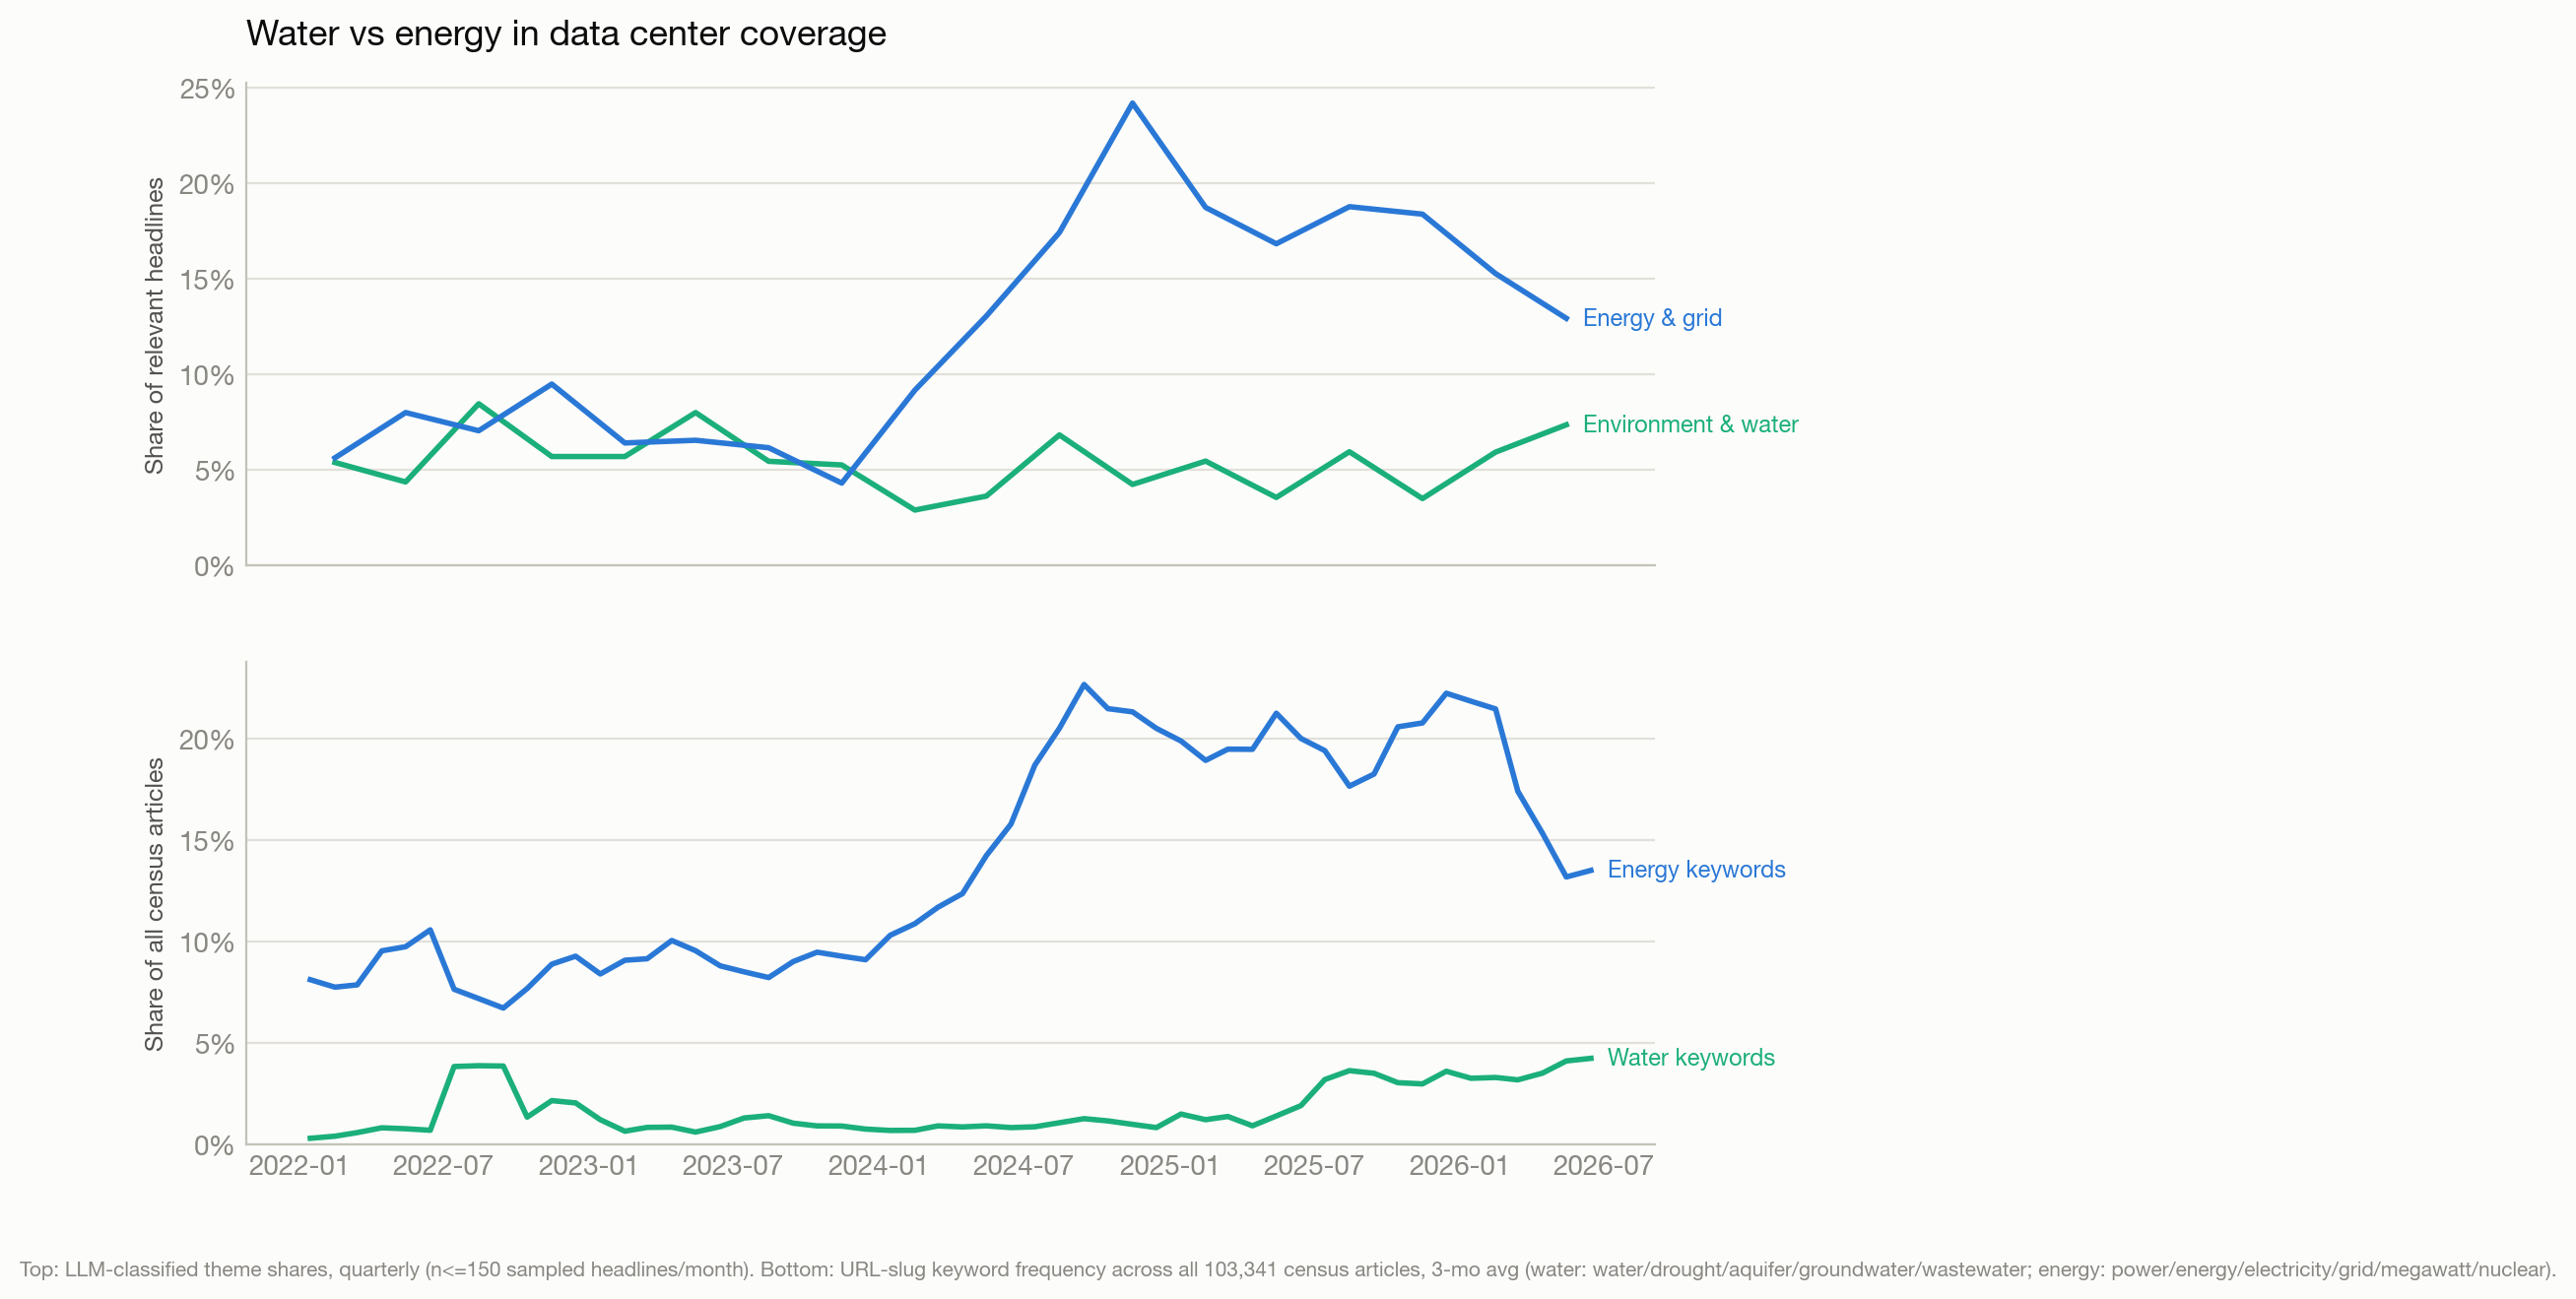
\includegraphics[width=\textwidth]{10_water_vs_energy.png}
\caption{Water versus energy in data center coverage. Top: classified theme
shares (quarterly). Bottom: keyword frequency in headline slugs across the
full census (monthly, smoothed).}
\label{fig:water}
\end{figure}

\section{Robustness}
\label{sec:robustness}

\textbf{Promotional-content filter.} As described above, the uniform filter
corrects a 22\%-promotional spike in 2025 cryptocurrency coverage and
strengthens the data center finding.

\textbf{Frame drift.} Late-period cryptocurrency coverage drifts toward AI
and data center usage of former mining facilities, which blurs that
comparison series after 2024; we caveat rather than correct this, as any
correction would require content-level judgments outside the rubric.

\textbf{Independent preliminary sample.} A preliminary fulltext-frame
sample (January--October 2022, about 30 relevant headlines per month)
yields a 2022 net sentiment of $+51$ points versus the census frame's
$+54$, indicating the headline result is not an artifact of frame choice.

\textbf{Measurement independence.} The LLM and lexicon measures agree at
$r=0.92$ quarterly on the series where change occurs
(Section~\ref{sec:calibration}).

\section{Limitations}
\label{sec:limitations}

Headlines are not articles: the classifier sees the headline and domain
only. The headline frame requires the term in the URL slug, excluding
stories about AI infrastructure that never name data centers. Coverage is
English-only. GDELT's source list over-represents wire and press-release
distributors, which we mitigate but cannot eliminate with the promotional
filter. For 28\% of sampled headlines (80\% in 2026) the title was
reconstructed from the URL slug; quality control found no systematic
sentiment effect, but confidence in 2026 monthly values is accordingly
lower. GDELT itself had outages on 2023-03-23 and 2025-06-15 through
2025-07-01. Finally, LLM classification is imperfect (87.2\% sentiment
agreement on re-classification); we publish all labels, prompts, and
rubrics so that any step can be audited or re-run.

\section{Discussion}

Read together, the results describe a technology buildout whose coverage
grew an order of magnitude while rotating from an investment story to a
community-impact story. The six-technology benchmark provides the relevant
context: turning negative is not unusual (four of six technologies did),
but the combination of depth (largest decline from a net-positive
baseline), breadth (the only technology whose local-outlet coverage went
sustainably net-negative in our outlet analysis), and duration (four
negative months and counting at the series end, where 5G and wind reverted
within two to four) is so far unique to data centers in this sample.

For infrastructure developers and their counterparties, the measurements
suggest three monitorable quantities: the recovery clock (whether national
sentiment reverts on the 5G/wind timescale or persists), the level of local
negative share (which reached 52\% in 2026-Q2 and moves contemporaneously
with national coverage), and water salience (small but growing faster than
any other environmental keyword we track). We offer these as descriptive
benchmarks rather than forecasts; the released pipeline updates monthly as
GDELT publishes.

\subsection*{Note added (July 19, 2026)}

Three developments after the close of our data window (June 2026) bear
directly on the measured trajectory and are noted here for completeness,
with sources. On July 18, 2026, 142 demonstrations concerning data center
construction were held across 42 U.S. states in a coordinated national day
of protest organized by the group HumansFirst, with participants
prominently citing water and electricity use \cite{reuters2026protests}. A
Reuters/Ipsos poll fielded in June 2026 ($n=4{,}531$) found 14\% of
American respondents comfortable with a data center being built near them,
and 57\% saying they would oppose one in their community
\cite{ipsos2026}. And on July 14, 2026, New York announced the first
statewide moratorium on new hyperscale (50\,MW and larger) data centers,
for up to one year pending a programmatic environmental review
\cite{nygov2026}. These events are consistent with the trajectory measured
here: community opposition as the largest negative theme, local-outlet
negative share above 50\%, and rising water salience. They fall outside
our measurement window and are not reflected in any series in this paper.

\section*{Data and code availability}

All code, SQL, prompts, classification rubrics, per-headline labels, and
processed series are available at
\url{https://github.com/ganesh-ketos/datacenter-media-sentiment}. Code is MIT
licensed; datasets, findings, and charts are released under CC BY 4.0 with
KETOS (\url{https://ketos.co}) as the designated attribution party, and the
underlying news metadata derive from the GDELT Project \cite{gdeltweb},
credited per its terms of use. All sampling and quality-control randomness
is seeded, and seeds are committed.

\begin{thebibliography}{9}

\bibitem{leetaru2013}
K.~Leetaru and P.~A. Schrodt,
``GDELT: Global data on events, location, and tone, 1979--2012,''
ISA Annual Convention, San Francisco, April 2013.

\bibitem{gdeltweb}
The GDELT Project, \url{https://www.gdeltproject.org/} (accessed July
2026).

\bibitem{claude}
Anthropic, ``Claude Sonnet'' (large language model),
\url{https://www.anthropic.com/} (2026).

\bibitem{reuters2026protests}
Reuters, ``Data center opponents stage 142 protests across 42 US states,''
July 18, 2026.

\bibitem{ipsos2026}
Ipsos, ``AI data centers are unpopular with most Americans,''
Reuters/Ipsos poll, June 2026,
\url{https://www.ipsos.com/en-us/ai-data-centers-are-unpopular-most-americans}.

\bibitem{nygov2026}
Office of the Governor of New York, ``First statewide moratorium on new
hyperscale data centers launched by Governor Kathy Hochul,'' July 14, 2026,
\url{https://www.governor.ny.gov/news/first-statewide-moratorium-new-hyperscale-data-centers-launched-governor-kathy-hochul}.

\end{thebibliography}

\end{document}
